\section{Implementation and Evaluation}
\label{sec:eval}

We describe in detail our implementation method and evaluation procedure for
answering  our goals using the patent dataset. The configuration of our
experimental desktop machine is RAM $16$ GB, 12 core with processor speed of
$2.8$ GHz Intel i7 and platform is Ubuntu $14.04$.

\begin{table*}[h] 
  %\centering
	\scriptsize
  \begin{tabular}{@{}c@{}} 
  \begin{minipage}{0.4\linewidth}
		\begin{center}
	  		\begin{tabular}{| l | l |}
				\hline
				
				{Type} & {Count} \\
				\hline
				\hline
				Inventors (Nodes) & 1222689 \\
				Co-authorships (Edges) & 3431064 \\
				Source Node & Thomas Edison\\
				\hline
			\end{tabular}		
			\caption {\scriptsize Details of the co-authorship graph}
			\label{tab:model}

			\vspace{0.85cm}

			\begin{tabular}{| l | l |}
				\hline
				{Algorithm} & {Time (sec)} \\
				\hline
				\hline
				Bellman-Ford & 0.80 \\
				Dijkstra & 1.28 \\
				Johnson & 1.29 \\
				\hline
			\end{tabular}
			\caption {\scriptsize Performance of the three shortest path algorithms}
			\label{tab:algos}
		\end{center}

  \end{minipage}
  \hspace{0.05\linewidth}
  \begin{minipage}{0.45\linewidth}
      \begin{figure}[H]
          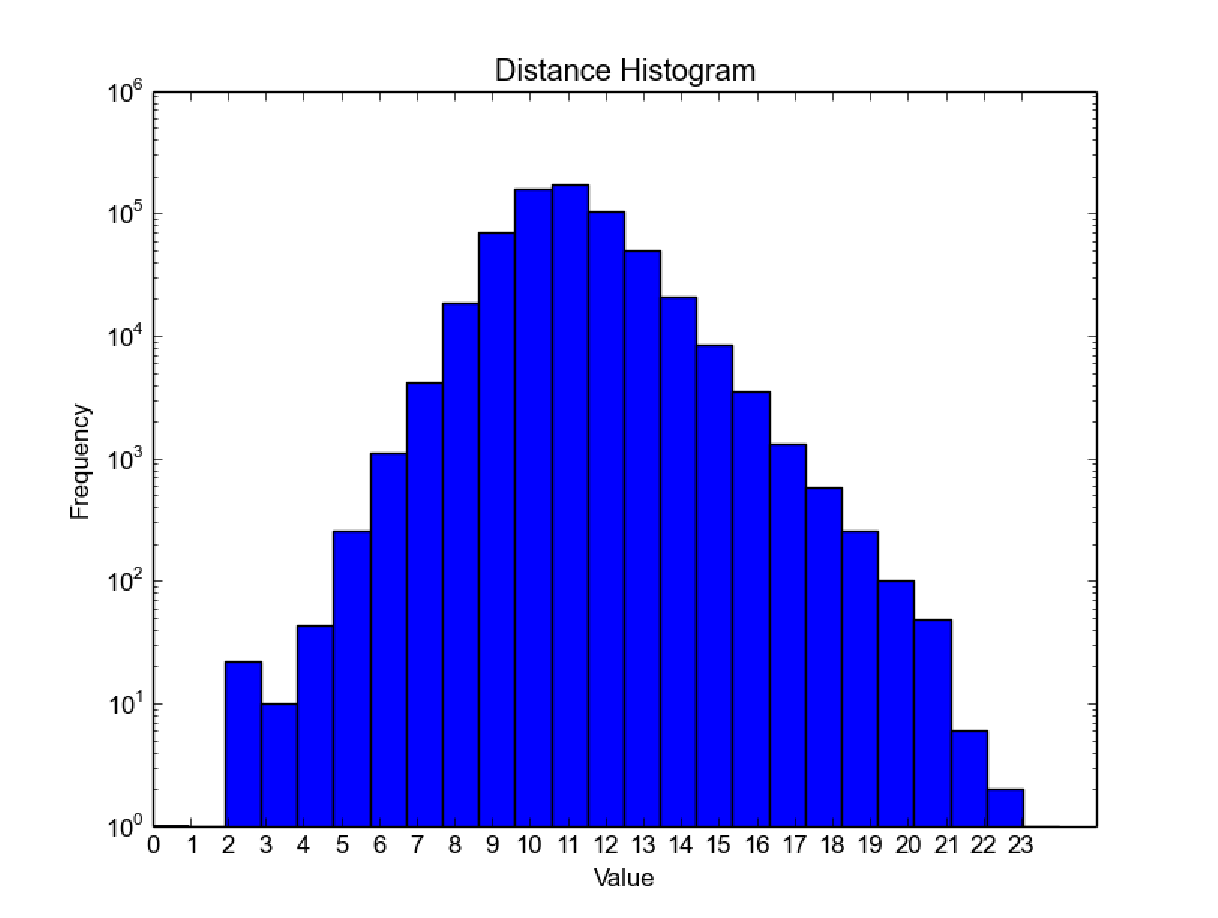
\includegraphics[scale=0.425]{../figures/distance.pdf}
          \caption{\scriptsize Graph shows the frequency of nodes on Y-axis and the distance from
		Edison on X-axis }
	  \label{fig:distance}
      \end{figure}
  \end{minipage}
  \end{tabular}
\end{table*}

% \end{minipage}

\begin{table*}[h] 
  %\centering
  \begin{tabular}{@{}c@{}} 
   \begin{minipage}{0.45\linewidth}
      \begin{figure}[H]
          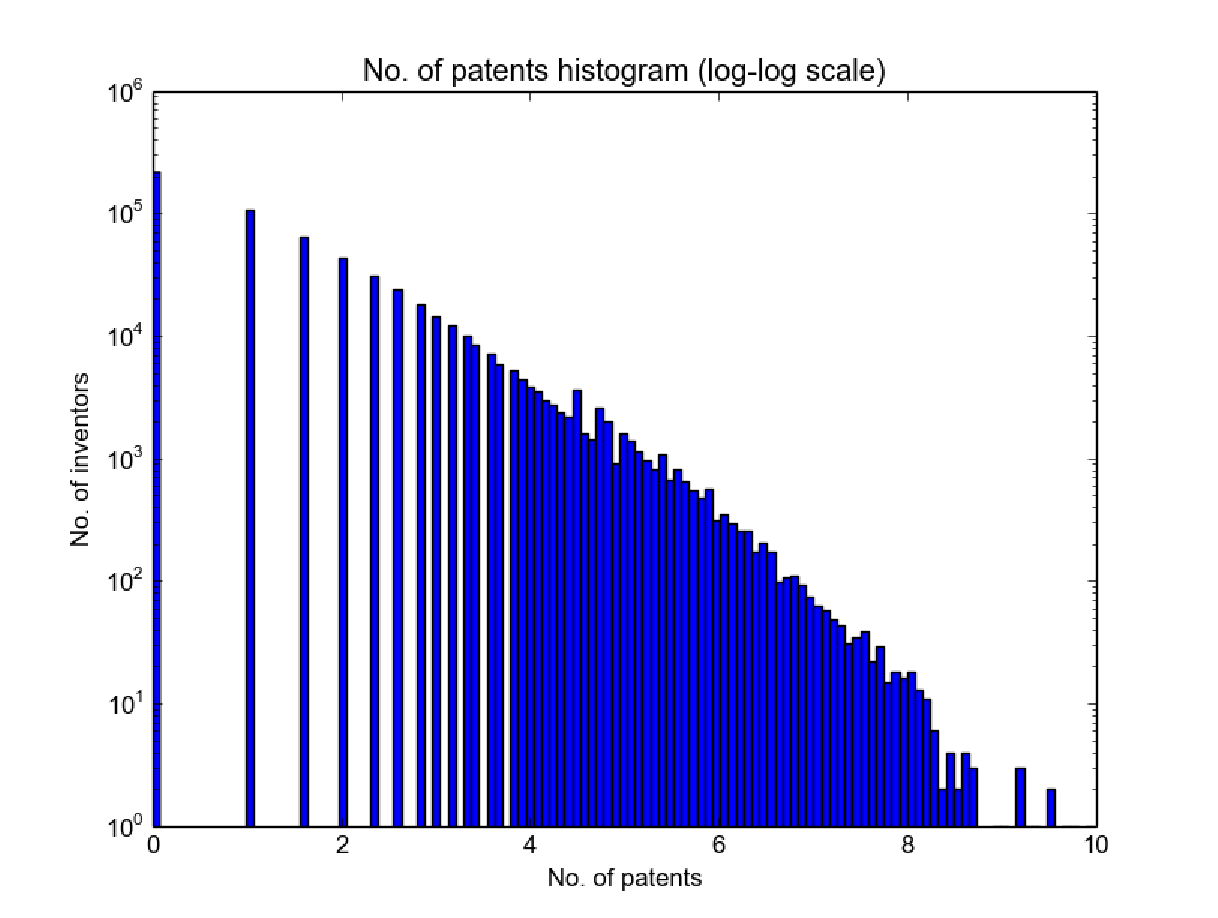
\includegraphics[scale=0.425]{../figures/patent.pdf}
          \caption{\scriptsize Log-log scale graph of no. of patents on Y-axis and the no.of inventors on X-axis}
	  \label{fig:patent}	
      \end{figure}
  \end{minipage}
  \begin{minipage}{0.45\linewidth}
      \begin{figure}[H]
          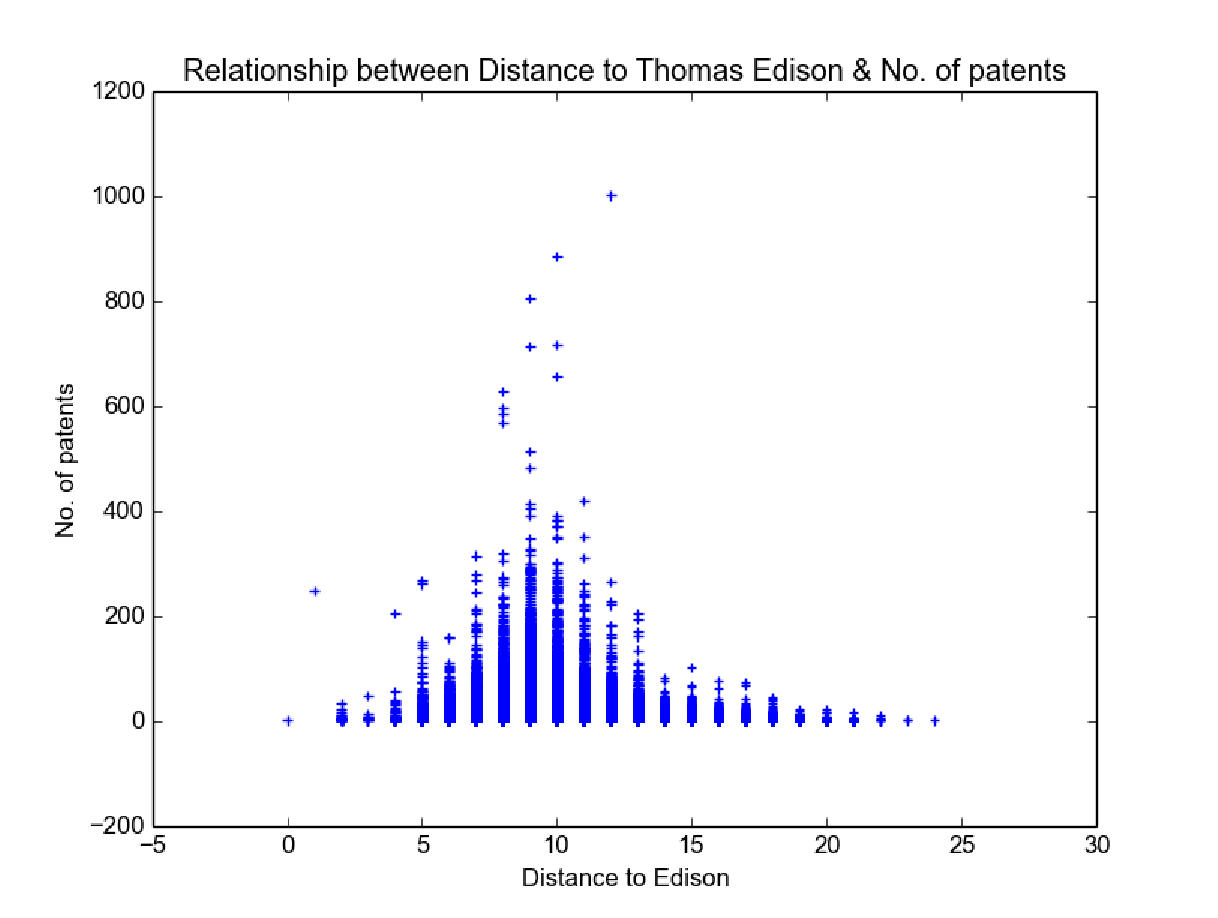
\includegraphics[scale=0.425]{../figures/distance_patent.pdf}
          \caption{\scriptsize Relationship graph of no. of patents of an inventor and his distance from Edison}
	  \label{fig:distance_patent}
      \end{figure}
  \end{minipage}
  \end{tabular}
\end{table*}

\subsection{Analysis Methodology}

\begin{itemize}
\squish
\item Gephi and / or IGraph: Graph analysis and metric calculation~\cite{gephi, igraph}.

\item GraphViz, Gnuplot: Data visualization and result plotting~\cite{graphviz, gnuplot}.

\item Standard libraries and custom Python Scripts: For data extraction~\cite{python}.
\end{itemize}

\subsection{Graph Details}
Table~\ref{tab:model} gives the details about Graph G1 in terms of its total
number of nodes , edges , patents, the source node  of the graph and the
average distance between the source node and all other nodes .    We choose
Thomas Edison as our source node as he is one of the top and popular inventors
in the patent dataset with maximum number of patents. We calculate the
shortest path of all other nodes from Thomas Edison.  We run three algorithms
particularly Djikstra shortest path algorithm, Bellman-ford and Johnson
available in IGraph tool on our Graph G1.


\subsection{Evaluation Steps}
	\begin{itemize}
		\squish
		\item {\em Evaluation Phase I - Collaborative Distance:} We calculated the 
		shortest path of each inventor w.r.t to Thomas Edison. We used three
		algorithms viz. Djikstra, Bellman-Ford, Johnson from IGraph to do this. We
		also analyzed their scalability with respect to the invention network graph
		and compared their performance.
		\item {\em Social Network Behavior:} Computed the distribution of the 
		collaborative distance w.r.t. Thomas Edison for our network, and also studied
		if the overall network follows power law for various popularity measures.
		\item {\em Evaluation Phase II - Eigenvalue centrality:} Use the Newman's
		leading eigenvector algorithm in IGraph to calculate eigenvalue centrality
		for each unique inventor with respect to patents that cite his / her patent.
		% ~\footnote{We skipped this activity for now, because it relies on the citation graph. Instead we did the next activity which uses the co-inventorship graph that we generated in this milestone.}.
		\item {\em Data analysis and comparison:} Plot the graphs for the above
		generated data and analyze the relationship between the above two
		measurements. Compare our ranking results for the most innovative organization
		with publicly available list such as Forbes list, to check if our ranking
		metric coincides with the results of other metrics.
	\end{itemize}

\subsection{Results}
Table~\ref{tab:algos} shows the execution time for each of the three shortest
path algorithms  when run on our graph G1. We observe that Djikstra's
algorithm takes $1.28$ seconds, Bellman-ford takes $0.80$ seconds and Johnson
algorithm takes $1.29$ seconds to run on our experimental setup.
Figure~\ref{fig:distance} shows the result for the total number of inventors
having the same distance from Edison. This graph follows a normal
distribution. Figure~\ref{fig:patent} shows the log-log graph of the total
no.of patents to total no.of inventors. We wil analyse whether this graph
follows the power law distribution in our  final analysis step.
Figure~\ref{fig:distance_patent} shows the relation of the distance from
Edison and the no. of patents for an inventor. This graph also follows a
normal distribution.
